\documentclass[9pt]{beamer}
\usepackage{ctex, hyperref}
\usepackage[T1]{fontenc}

\usepackage{latexsym,amsmath,xcolor,multicol,booktabs,calligra}
\usepackage{graphicx,pstricks,listings,stackengine}
\usepackage[style=gb7714-2015,backend=biber]{biblatex}
\addbibresource{reference.bib}
\usepackage{tikz}
\usepackage{algorithm}
\usepackage{algpseudocode}
\usepackage{palatino}
\usepackage{caption}
\usefonttheme[onlymath]{serif}

\usetikzlibrary{arrows, shapes.geometric}
\tikzstyle{process} = [rectangle, minimum width=3cm, minimum height=1cm, text centered, draw=black]
\tikzstyle{arrow} = [thick,->,>=stealth]
\usepackage{multirow}
\setbeamertemplate{bibliography item}[text]

\author{张珂,周吉林}
\title{考虑企业社会责任的应急物资协同储备:Stackelberg博弈模型}
\subtitle{论文汇报}
\institute{北京邮电大学 智能工程与自动化学院}
\date{\today}
\usepackage{College}

\def\cmd#1{\texttt{\color{red}\footnotesize $\backslash$#1}}
\def\env#1{\texttt{\color{blue}\footnotesize #1}}
\definecolor{deepblue}{rgb}{0,0,0.5}
\definecolor{deepred}{rgb}{0.6,0,0}
\definecolor{deepgreen}{rgb}{0,0.5,0}
\definecolor{halfgray}{gray}{0.55}

\lstset{
    basicstyle=\ttfamily\small,
    keywordstyle=\bfseries\color{deepblue},
    emphstyle=\ttfamily\color{deepred},
    stringstyle=\color{deepgreen},
    numbers=left,
    numberstyle=\small\color{halfgray},
    rulesepcolor=\color{red!20!green!20!blue!20},
    frame=shadowbox,
}

\begin{document}

\kaishu
\begin{frame}
    \titlepage
    \begin{figure}[htpb]
        \begin{center}
            \vspace*{-0.5cm}
            
\includegraphics[width=0.18\linewidth]{basic_pictures/bupt.jpg}
        \end{center}
    \end{figure}
\end{frame}

\begin{frame}{目录}
\tableofcontents[sectionstyle=show,subsectionstyle=show/shaded/hide,subsubsectionstyle=show/shaded/hide]
\end{frame}

\section{背景介绍}
\begin{frame}{\insertsectionhead: 研究背景与意义}
    \begin{itemize}
        \item 我国自然灾害频发,应急物资储备至关重要 \cite{MEM2024disaster, chen2009modern}。
        \item 传统储备模式问题:物资单一、成本高、效率低 \cite{chen2014突发事件灾前应急物资政企联合储备模式, wang2023防汛物资}。
        \item 国家政策导向:构建政企协同、实物与产能结合的储备模式 \cite{ndrc2022, sfdrrmc2024}。
        \item 强调应急物流社会化 \cite{lu2009应急物资储备的社会化研究}。
    \end{itemize}
    \begin{figure}
        \centering
        
\includegraphics[width=0.8\linewidth]{basic_pictures/政府文件.png}
        \caption{相关政策文件}
        \label{fig:beamer_policy_guidance}
    \end{figure}
\end{frame}
% 放张图片

% 做成表展示
\begin{frame}{\insertsectionhead: 文献回顾}
    \begin{itemize}
        \item \textbf{博弈论应用:}
            \begin{itemize}
                \item Stackelberg博弈模型分析政企合作 \cite{Li2022Stackelberg}。
                \item 演化博弈模型分析多方参与 \cite{Zhang2022Evolutionary, shao2023非常规突发事件}。
                \item 国际研究关注激励与协调机制 \cite{egan2010private, balcik2010coordination, vanwyk2011modeling, coskun2019relief}。
            \end{itemize}
        \item \textbf{契约机制设计:}
            \begin{itemize}
                \item 期权契约降低决策风险 \cite{rabbani2015option, wang2015prepurchasing, Pang2020PhysicalOption}。
                \item 数量柔性契约协调供需 \cite{nikkhoo2018coordination, chai2021考虑储备周期}。
                \item 多企业参与的复杂契约 \cite{Chen2023Contract, Li2024CooperationStrategies}。
                \item 期权契约理论基础 \cite{black1973pricing, barnes2002coordination, xu2010managing}。
            \end{itemize}
        \item \textbf{其他关键因素与复杂供应链:}
            \begin{itemize}
                \item 三级供应链与数量柔性契约 \cite{Gong2024Quantity}。
                \item 人道主义供应链整体优化 \cite{torabi2018integrated}。
                \item 企业社会责任(CSR)融入模型 \cite{zhengh2023}。
                \item 物资维护水平 \cite{wang2023考虑维护水平}。
                \item 生产能力储备 \cite{hu2018考虑企业生产能力, zhang2016emergency}。
                \item 多级供应链与代储模式 \cite{jiang2024基于代储模式}。
            \end{itemize}
    \end{itemize}
\end{frame}

\begin{frame}{\insertsectionhead: 现有研究不足与本文贡献}
    \textbf{现有研究不足:}
    \begin{itemize}
        \item 企业社会责任(CSR)考量不足:多将企业视为纯粹逐利者 \cite{Li2022Stackelberg, Chen2023Contract},忽视利他行为 \cite{zhengh2023}。
        \item 需求分布假设简化:多采用均匀分布 \cite{chai2021考虑储备周期, chen2014突发事件灾前应急物资政企联合储备模式},与现实差异大。
        \item 多样化储备方式协同研究不足:多单独研究物资储备 \cite{Li2022Stackelberg, li2022政企联合储备, Chen2023Contract} 或产能储备 \cite{Gong2024Quantity},企业捐赠协同效应研究空白。
    \end{itemize}
    \textbf{本文研究目的与贡献:}
    \begin{itemize}
        \item 构建更全面且贴近现实的政企联合应急物资储备决策模型。
        \item 考虑企业社会责任、多种储备方式协同及更真实的需求分布。
    \end{itemize}
\end{frame}

\section{模型构建}
\begin{frame}{\insertsectionhead: 模型框架}
    \begin{itemize}
        \item \textbf{参与主体:} 政府 (领导者),企业 (跟随者) - Stackelberg 博弈 \cite{Li2022Stackelberg}。
        \item \textbf{储备方式:}
            \begin{enumerate}
                \item 政府实物储备 ($Q$)
                \item 企业实物储备 ($q$)
                \item 企业捐赠 ($Q_j$) (考虑企业社会责任)
                \item 企业生产能力储备
            \end{enumerate}
    \end{itemize}
    \begin{figure}
        \centering
        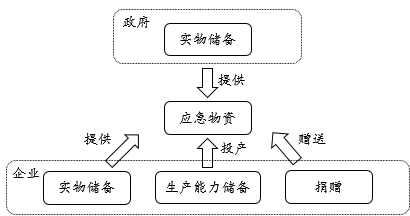
\includegraphics[width=0.6\linewidth]{basic_pictures/结构图.png}
        \caption{多主体协同应急物资储备计划示意}
    \end{figure}
\end{frame}

\begin{frame}{\insertsectionhead: 前提与假设}
    \begin{enumerate}
        \item \textbf{物资调用顺序:} 政府实物储备 $\rightarrow$ 企业实物储备 $\rightarrow$ 企业捐赠物资 $\rightarrow$ 企业生产能力储备。
        \item \textbf{物资保质期:} 储备周期小于保质期,期末残值 $v$ 轮换。
        \item \textbf{政府协同前提:} $p_1 + c_1 - v - p_2 > 0$。
        \item \textbf{企业参与激励:} $s > v$ 且 $m > s + p_2$。
    \end{enumerate}
\end{frame}

\begin{frame}{\insertsectionhead: 应急物资需求概率分布}
    \begin{itemize}
        \item 传统模型多采用均匀分布 \cite{chai2021考虑储备周期,chen2014突发事件灾前应急物资政企联合储备模式,hu2018考虑企业生产能力}:
            \begin{equation} \label{eq:beamer_uniform_cdf}
            F(x) = \begin{cases}
            0 & x < 0 \\
            \frac{x}{U} & 0 \leq x \leq U \\
            1 & x > U
            \end{cases}
            \end{equation}
        \item 本文后续算例将采用基于历史数据拟合的反高斯分布,以更贴近现实。
    \end{itemize}
\end{frame}

\begin{frame}{\insertsectionhead: 政府方期望收益}
    灾害未发生时($1-\alpha$)政府利润 ($\pi_{g,0}$):
    \begin{equation} \label{eq:beamer_profit_no_disaster_gov}
    \pi_{g,0}(Q,q) = v Q - (p_1 + c_1) Q - p_2 q
    \end{equation}
    灾害发生时($\alpha$)政府利润 ($\pi_{g,\alpha}$),考虑四种需求情况:
    \begin{itemize}
        \item $0 < x \leq Q$: $v(Q-x) - (p_1+c_1)Q - p_2q$
        \item $Q < x \leq Q+q$: $-(p_1+c_1)Q - p_2q - s(x-Q)$
        \item $Q+q < x \leq Q+q+Q_j$: $-(p_1+c_1)Q - p_2q - sq$
        \item $Q+q+Q_j < x \leq U$: $-(p_1+c_1)Q - p_2q - sq - m(x-Q-q-Q_j)$
    \end{itemize}
    政府总期望利润 ($\pi_g(Q,q)$):
    \begin{equation} \label{eq:beamer_expected_profit_gov}
    \pi_g(Q,q) = (1-\alpha) \pi_{g,0}(Q,q) + \alpha \pi_{g,\alpha}(Q,q, Q_j)
    \end{equation}
    
\end{frame}

\begin{frame}{\insertsectionhead: 企业期望收益}
    灾害未发生时($1-\alpha$)企业利润 ($\pi_{r,0}$):
    \begin{equation} \label{eq:beamer_enterprise_profit_no_disaster}
    {\pi}_{r,0}(q) = (v + p_2 - c_2)q
    \end{equation}
    灾害发生时($\alpha$)企业利润 ($\pi_{r,\alpha}$),考虑四种物资调用阶段。
    \begin{itemize}
        \item $0 < x \leq Q$: $(v + p_2 - c_2)q$
        \item $Q < x \leq Q+q$: $s(x-Q) + v(Q + q - x) + (p_2 - c_2)q$
        \item $Q+q < x \leq Q+q+Q_j$: $sq + (p_2 - c_2)q + \lambda(m-e)\sqrt{Q_jm} - eQ_j$
        \item $x > Q+q+Q_j$: $sq + (p_2 - c_2)q + \lambda(m-e)\sqrt{Q_jm} - eQ_j + (m-e)(x-Q-q-Q_j)$
    \end{itemize}
    企业总期望利润 (${\pi}_r(Q_j,q)$):
    \begin{equation} \label{eq:beamer_enterprise_expected_profit}
    {\pi}_r(Q_j,q) = (1-\alpha){\pi}_{r,0}(q) + \alpha{\pi}_{r,\alpha}(Q_j,q)
    \end{equation}
   
\end{frame}

\section{模型求解}
\begin{frame}{\insertsectionhead: Stackelberg博弈与求解思路}
    \begin{itemize}
        \item \textbf{博弈框架:} 政府为领导者,企业为跟随者。
        \item \textbf{求解方法:} 逆向归纳法 \cite{balcik2010coordination}。
            \begin{enumerate}
                \item 企业在给定政府决策 $Q$ 后,最大化自身收益,确定 $q^*(Q)$ 和 $Q_j^*(Q)$。
                \item 政府预测到企业响应,最大化自身收益,确定 $Q^*$。
            \end{enumerate}
    \end{itemize}
    \begin{figure}
    \centering
    \begin{tikzpicture}[node distance=1.3cm, scale=0.9, transform shape]
    \node (gov) [process, minimum width=2.5cm, minimum height=0.8cm] {政府确定$Q$};
    \node (firm) [process, below of=gov, minimum width=2.5cm, minimum height=0.8cm] {企业确定$q^*(Q), Q_j^*(Q)$};
    \node (gov_solve) [process, below of=firm, node distance=1.8cm, minimum width=2.5cm, minimum height=0.8cm] {政府求解最优$Q^*$};
    \node (equilibrium) [process, below of=gov_solve, minimum width=2.5cm, minimum height=0.8cm] {Stackelberg均衡};
    \draw [arrow] (gov) -- node[anchor=west, xshift=0.1cm] {\footnotesize 发布 $Q$} (firm);
    \draw [arrow] (firm) -- node[anchor=west, xshift=0.1cm] {\footnotesize 响应 $q^*(Q), Q_j^*(Q)$} (gov_solve);
    \draw [arrow] (gov_solve) -- (equilibrium);
    \end{tikzpicture}
    \caption{Stackelberg博弈求解流程}
    \label{fig:beamer_solution_process}
    \end{figure}
\end{frame}

\begin{frame}{\insertsectionhead: 企业最优响应}
    \textbf{1. 确定最优捐赠量 $Q_j^*$}
    \begin{itemize}
        \item 对 $\pi_r(Q_j,q)$ 关于 $Q_j$ 求一阶偏导数 $\frac{\partial{\pi}_r}{\partial Q_j}$。
        \item 二阶偏导数 $\frac{\partial^2 {\pi}_r}{\partial Q_j^2} < 0$, 表明 $\pi_r$ 是 $Q_j$ 的严格凹函数。
        \item 最优捐赠量 $Q_j^*$ (由 $\frac{\partial{\pi}_r}{\partial Q_j}=0$ 且 $f(Q+q+Q_j) \approx 0$ 近似得到):
        \begin{equation} \label{eq:beamer_optimal_Qj}
        Q_j^* = \frac{\lambda^2 m (m-e)^2}{4e^2}
        \end{equation}
        此 $Q_j^*$ 不依赖于 $Q$ 和 $q$。
    \end{itemize}
    \vspace{0.5em}
    \textbf{2. 确定最优储备量 $q^*$}
    \begin{itemize}
        \item 对 $\pi_r(Q,q)$ 关于 $q$ 求一阶偏导数 $\frac{\partial \pi_r(Q,q)}{\partial q}$。
        \item 结果显示 $\frac{\partial \pi_r(Q,q)}{\partial q} > 0$ 恒成立。
        \item \textbf{结论:} 企业期望利润随 $q$ 单调递增。在政府引导或设定企业储备量 $q$ 的框架下,企业最优响应是执行政府设定的 $q$ 值。
    \end{itemize}
f\end{frame}

\begin{frame}{\insertsectionhead: 政府最优决策}
    \begin{itemize}
        \item 政府目标:最大化期望利润 $\pi_g(Q,q)$。
        \item 决策变量:$Q$ (政府实物储备) 和 $q$ (对企业的储备要求)。
        \item 约束条件:$Q \ge 0, q \ge 0, Q \ge q$。
        \item Hessian矩阵分析:
            \begin{itemize}
                \item $\frac{\partial^2 \pi_g(Q,q)}{\partial Q^2} \frac{\partial^2 \pi_g(Q,q)}{\partial q^2} - \left(\frac{\partial^2 \pi_g(Q,q)}{\partial Q\partial q}\right)^2 > 0$
                \item 表明政府利润函数是 $Q$ 和 $q$ 的凹函数,最大值存在。
            \end{itemize}
        \item 模型复杂,无法获得 $Q, q$ 的显式解,需采用数值方法。
    \end{itemize}
\end{frame}

\begin{frame}{\insertsectionhead: 序列最小二乘二次规划 (SLSQP) 算法}
    \begin{itemize}
        \item \textbf{适用性:} 求解带约束的非线性规划问题,无需显式Hessian矩阵。
        \item \textbf{核心思想:} 迭代求解二次规划子问题。
    \end{itemize}
    \textbf{SLSQP算法流程概述:}
    \begin{algorithmic}[1]
        \State \textbf{输入:} 初始点 $x_0$, 允许误差 $\varepsilon$, 最大迭代次数 $K$
        \State \textbf{初始化:} $k \leftarrow 0$, $B_0 \leftarrow I$
        \While{$k < K$ \textbf{and} 未收敛}
            \State 计算 $f(x_k), \nabla f(x_k), c_i(x_k), \nabla c_i(x_k)$
            \State 求解QP子问题得搜索方向 $d_k$ 
            \State 线搜索确定步长 $\alpha_k$ 
            \State 更新 $x_{k+1} \leftarrow x_k + \alpha_k d_k$
            \State 更新Hessian近似 $B_{k+1}$ 
            \State 判断收敛
            \State $k \leftarrow k + 1$
        \EndWhile
        \State \textbf{输出:} 近似最优解 $x_k$
    \end{algorithmic}
\end{frame}

% 添加一页介绍更新方法
\begin{frame}{SLSQP 算法核心更新公式}
    \framesubtitle{补充说明}
    以下为SLSQP算法中关键步骤的更新公式:
    \vspace{0.5em}
    \textbf{1. 求解搜索方向 $d_k$ (二次规划子问题):}
    \begin{align*}
        \min_{d} \quad & \nabla f(x_k)^T d + \frac{1}{2}d^T B_k d \\
        \text{s.t.} \quad & c_i(x_k) + \nabla c_i(x_k)^T d = 0, \quad i \in \mathcal{E} \\
        & c_i(x_k) + \nabla c_i(x_k)^T d \geq 0, \quad i \in \mathcal{I} \\
        & l \leq x_k + d \leq u
    \end{align*}
    其中 $B_k$ 是Hessian矩阵的近似。
    
    \textbf{2. 线搜索确定步长 $\alpha_k$ (Wolfe 条件):}
    \begin{align*}
        & f(x_k + \alpha_k d_k) \leq f(x_k) + c_1 \alpha_k \nabla f(x_k)^T d_k \\
        & |\nabla f(x_k + \alpha_k d_k)^T d_k| \leq c_2 |\nabla f(x_k)^T d_k|
    \end{align*}
    其中 $0 < c_1 < c_2 < 1$ 为常数。
 
    
\end{frame}

\begin{frame}{SLSQP算法核心更新公式}
    \textbf{3. 更新Hessian近似 $B_{k+1}$:}
    \begin{itemize}
        \item 计算位移 $s_k$ 和梯度差 $y_k$:
            \begin{align*}
            s_k &= x_{k+1} - x_k \\
            y_k &= \nabla \mathcal{L}(x_{k+1}, \lambda_k) - \nabla \mathcal{L}(x_k, \lambda_k)
            \end{align*}
        \item 其中,拉格朗日函数 $\mathcal{L}(x, \lambda)$ 定义为:
            \begin{equation*}
            \mathcal{L}(x, \lambda) = f(x) - \sum_{i \in \mathcal{E} \cup \mathcal{I}} \lambda_i c_i(x)
            \end{equation*}
        \item $B_{k+1}$ 通常使用 $s_k$ 和 $y_k$ 通过拟牛顿法(如BFGS)更新,SLSQP采用最小二乘技术估计。
    \end{itemize}

\end{frame}

\section{算例分析}
\begin{frame}{\insertsectionhead: 算例情景与参数设置}
    \textbf{单位应急物资构成参考:}《全国基础版家庭应急物资储备建议清单》\cite{china_emergency_management_2020}。
    \begin{itemize}
        \item 饮用水、罐头、压缩饼干、手电筒、小刀、医疗用品等。
        \item 单位应急物资灾前采购成本 ($p_1$) 设定为 220元。
    \end{itemize}
    \begin{table}
    \centering
    \caption{算例参数设置}
\small
    \begin{tabular}{llcl}
    \toprule
    参数符号 & 参数含义                     & 数值    & 单位 \\
    \midrule
    $p_1$      & 单位应急物资灾害前采购成本   & 220 & 元   \\
    $v$        & 单位物资残值                 & 150   & 元   \\
    $m$        & 灾害后应急物资市场单价       & 500   & 元   \\
    $\alpha$   & 灾害发生概率                 & 1     & -    \\
    $e$        & 企业单位物资加急生产成本     & 400   & 元   \\
    $p_2$      & 企业单位物资代储收入         & 170   & 元   \\
    $c_2$      & 企业单位物资储存成本         & 300    & 元   \\
    $s$        & 企业单位物资使用补贴         & 180   & 元   \\
    $c_1$      & 政府单位物资储存成本         & 120   & 元   \\
    $\lambda$  & 企业捐赠行为影响系数         & 0.2   & -    \\
    $U$        & 最大物资需求量               & 15 & 万 \\
    \bottomrule
    \end{tabular}
    \end{table}
    参数设置满足模型假设条件。
\end{frame}

\begin{frame}{\insertsectionhead: 需求概率分布建模}
    \begin{itemize}
        \item \textbf{数据来源:} EM-DAT数据库 (1900-2022年中国洪涝灾害)。
        \item \textbf{拟合方法:} 对历史需求数据进行概率分布拟合与检验。
    \end{itemize}
    \begin{table}
    \centering
    \caption{不同概率分布拟合统计量比较}
        \small
\begin{tabular}{cccc}
    \toprule
    分布类型    & SSE ($10^{-13}$) & AIC        & BIC \\
    \midrule
    逆高斯分布 & \textbf{6.57}    & 4028.48    & 4039.04\\
    对数正态分布 & 10.34            & \textbf{3928.83}    & \textbf{3939.38}\\
    Burr分布      & 9.00             & 3951.92    & 3965.99   \\
    帕累托分布   & 8.21             & 3970.38    & 3980.94   \\
    贝塔分布      & 13.17            & 4192.39    & 4206.46   \\
    \bottomrule
    \end{tabular}
    \end{table}
    \textbf{结论:} 反高斯分布的SSE最小,拟合效果较好。
    \begin{equation} \label{eq:beamer_pdf_demand}
    f(x) = \sqrt{\frac{4.87}{2\pi (x + 0.97)^3}} e^{\left[ -\frac{4.87 \left((x + 0.97) - 40.69\right)^2}{2(40.69)^2 (x + 0.97)} \right]}
    \end{equation}
\end{frame}

% \begin{frame}{\insertsectionhead: 需求分布拟合结果}
%     \begin{figure}
%         \centering
%         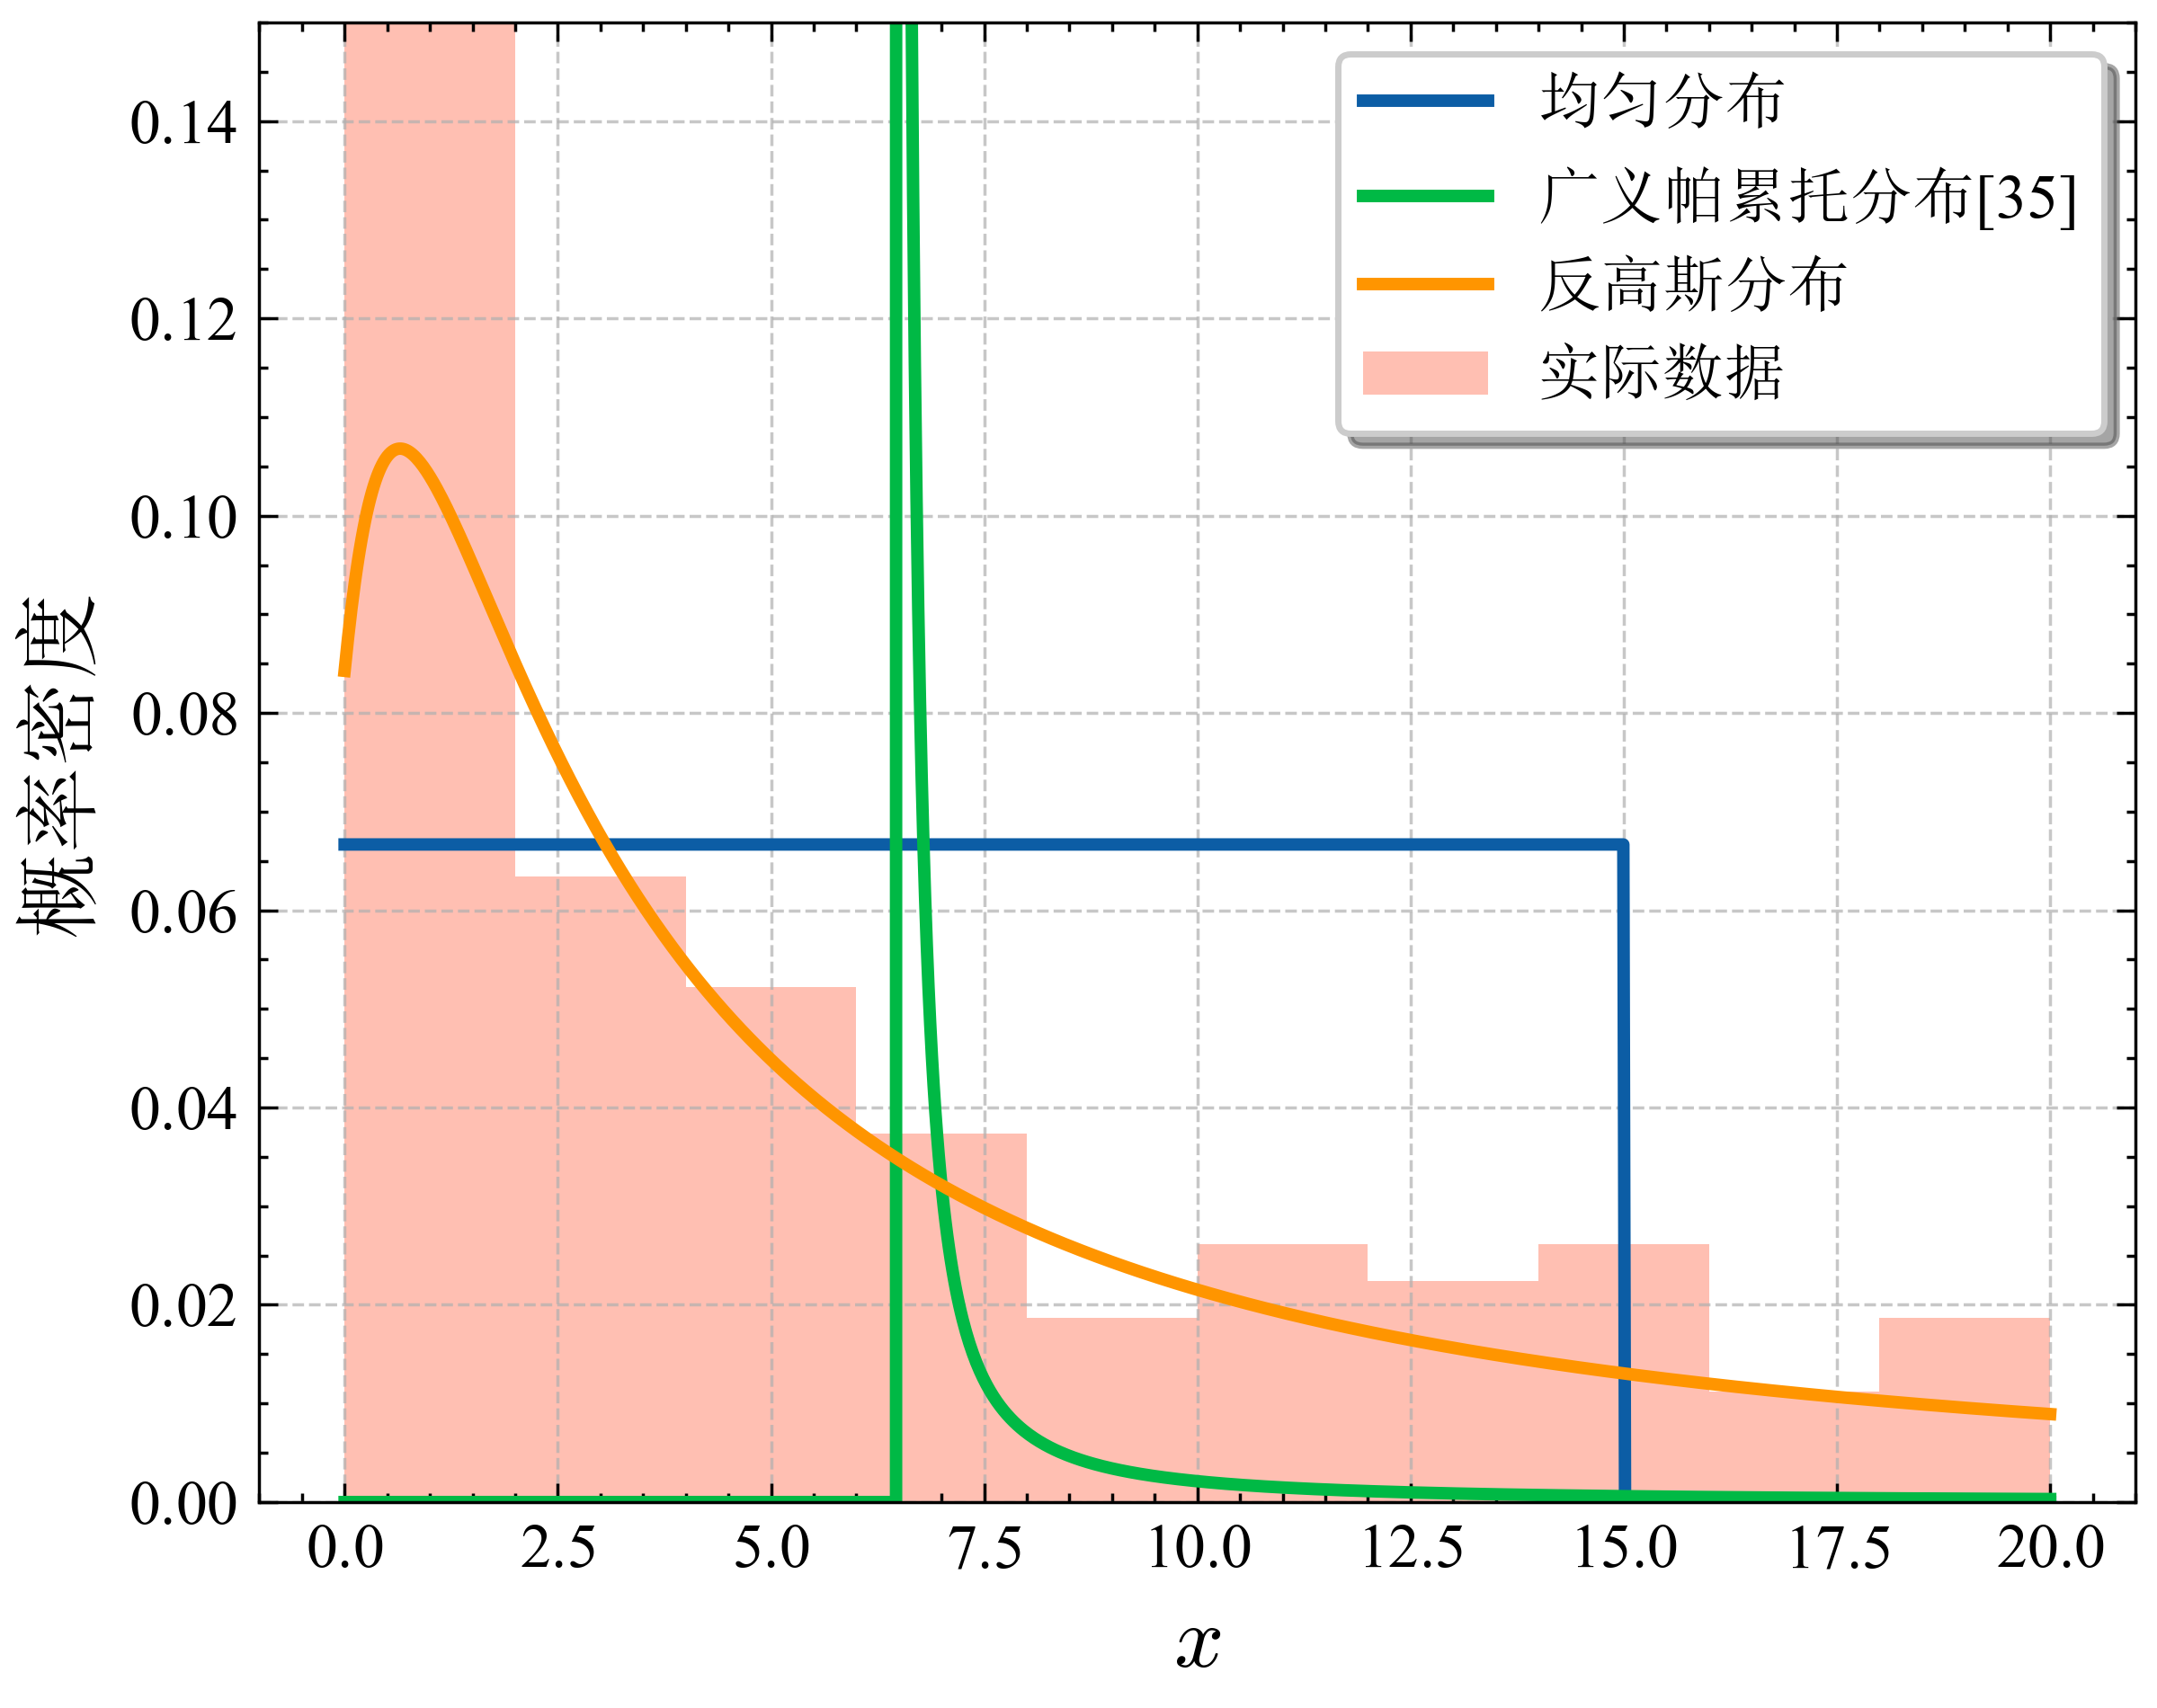
\includegraphics[width=0.7\linewidth]{basic_pictures/分布拟合.png}
%         \caption{分布拟合结果}
%         \label{fig:beamer_dist_fit}
%     \end{figure}
%     \begin{itemize}
%         \item 实际数据呈右偏分布,小需求概率高。
%         \item 反高斯分布 (橙色) 较好地拟合了实际数据形态,优于均匀分布 (蓝色) 和广义帕累托分布 (绿色) \cite{Li2022Stackelberg}。
%     \end{itemize}
% \end{frame}

\begin{frame}{\insertsectionhead: 需求分布拟合结果}
    \begin{columns}
        % 左侧文字列,占0.5的宽度
        \begin{column}{0.5\textwidth}
            \begin{itemize}
                \item 实际数据呈右偏分布,小需求概率高。
                \item 反高斯分布 (橙色) 较好地拟合了实际数据形态,优于均匀分布 (蓝色) 和广义帕累托分布 (绿色) \cite{Li2022Stackelberg}。
            \end{itemize}
        \end{column}
        
        % 右侧图像列,占0.5的宽度
        \begin{column}{0.5\textwidth}
            \centering
            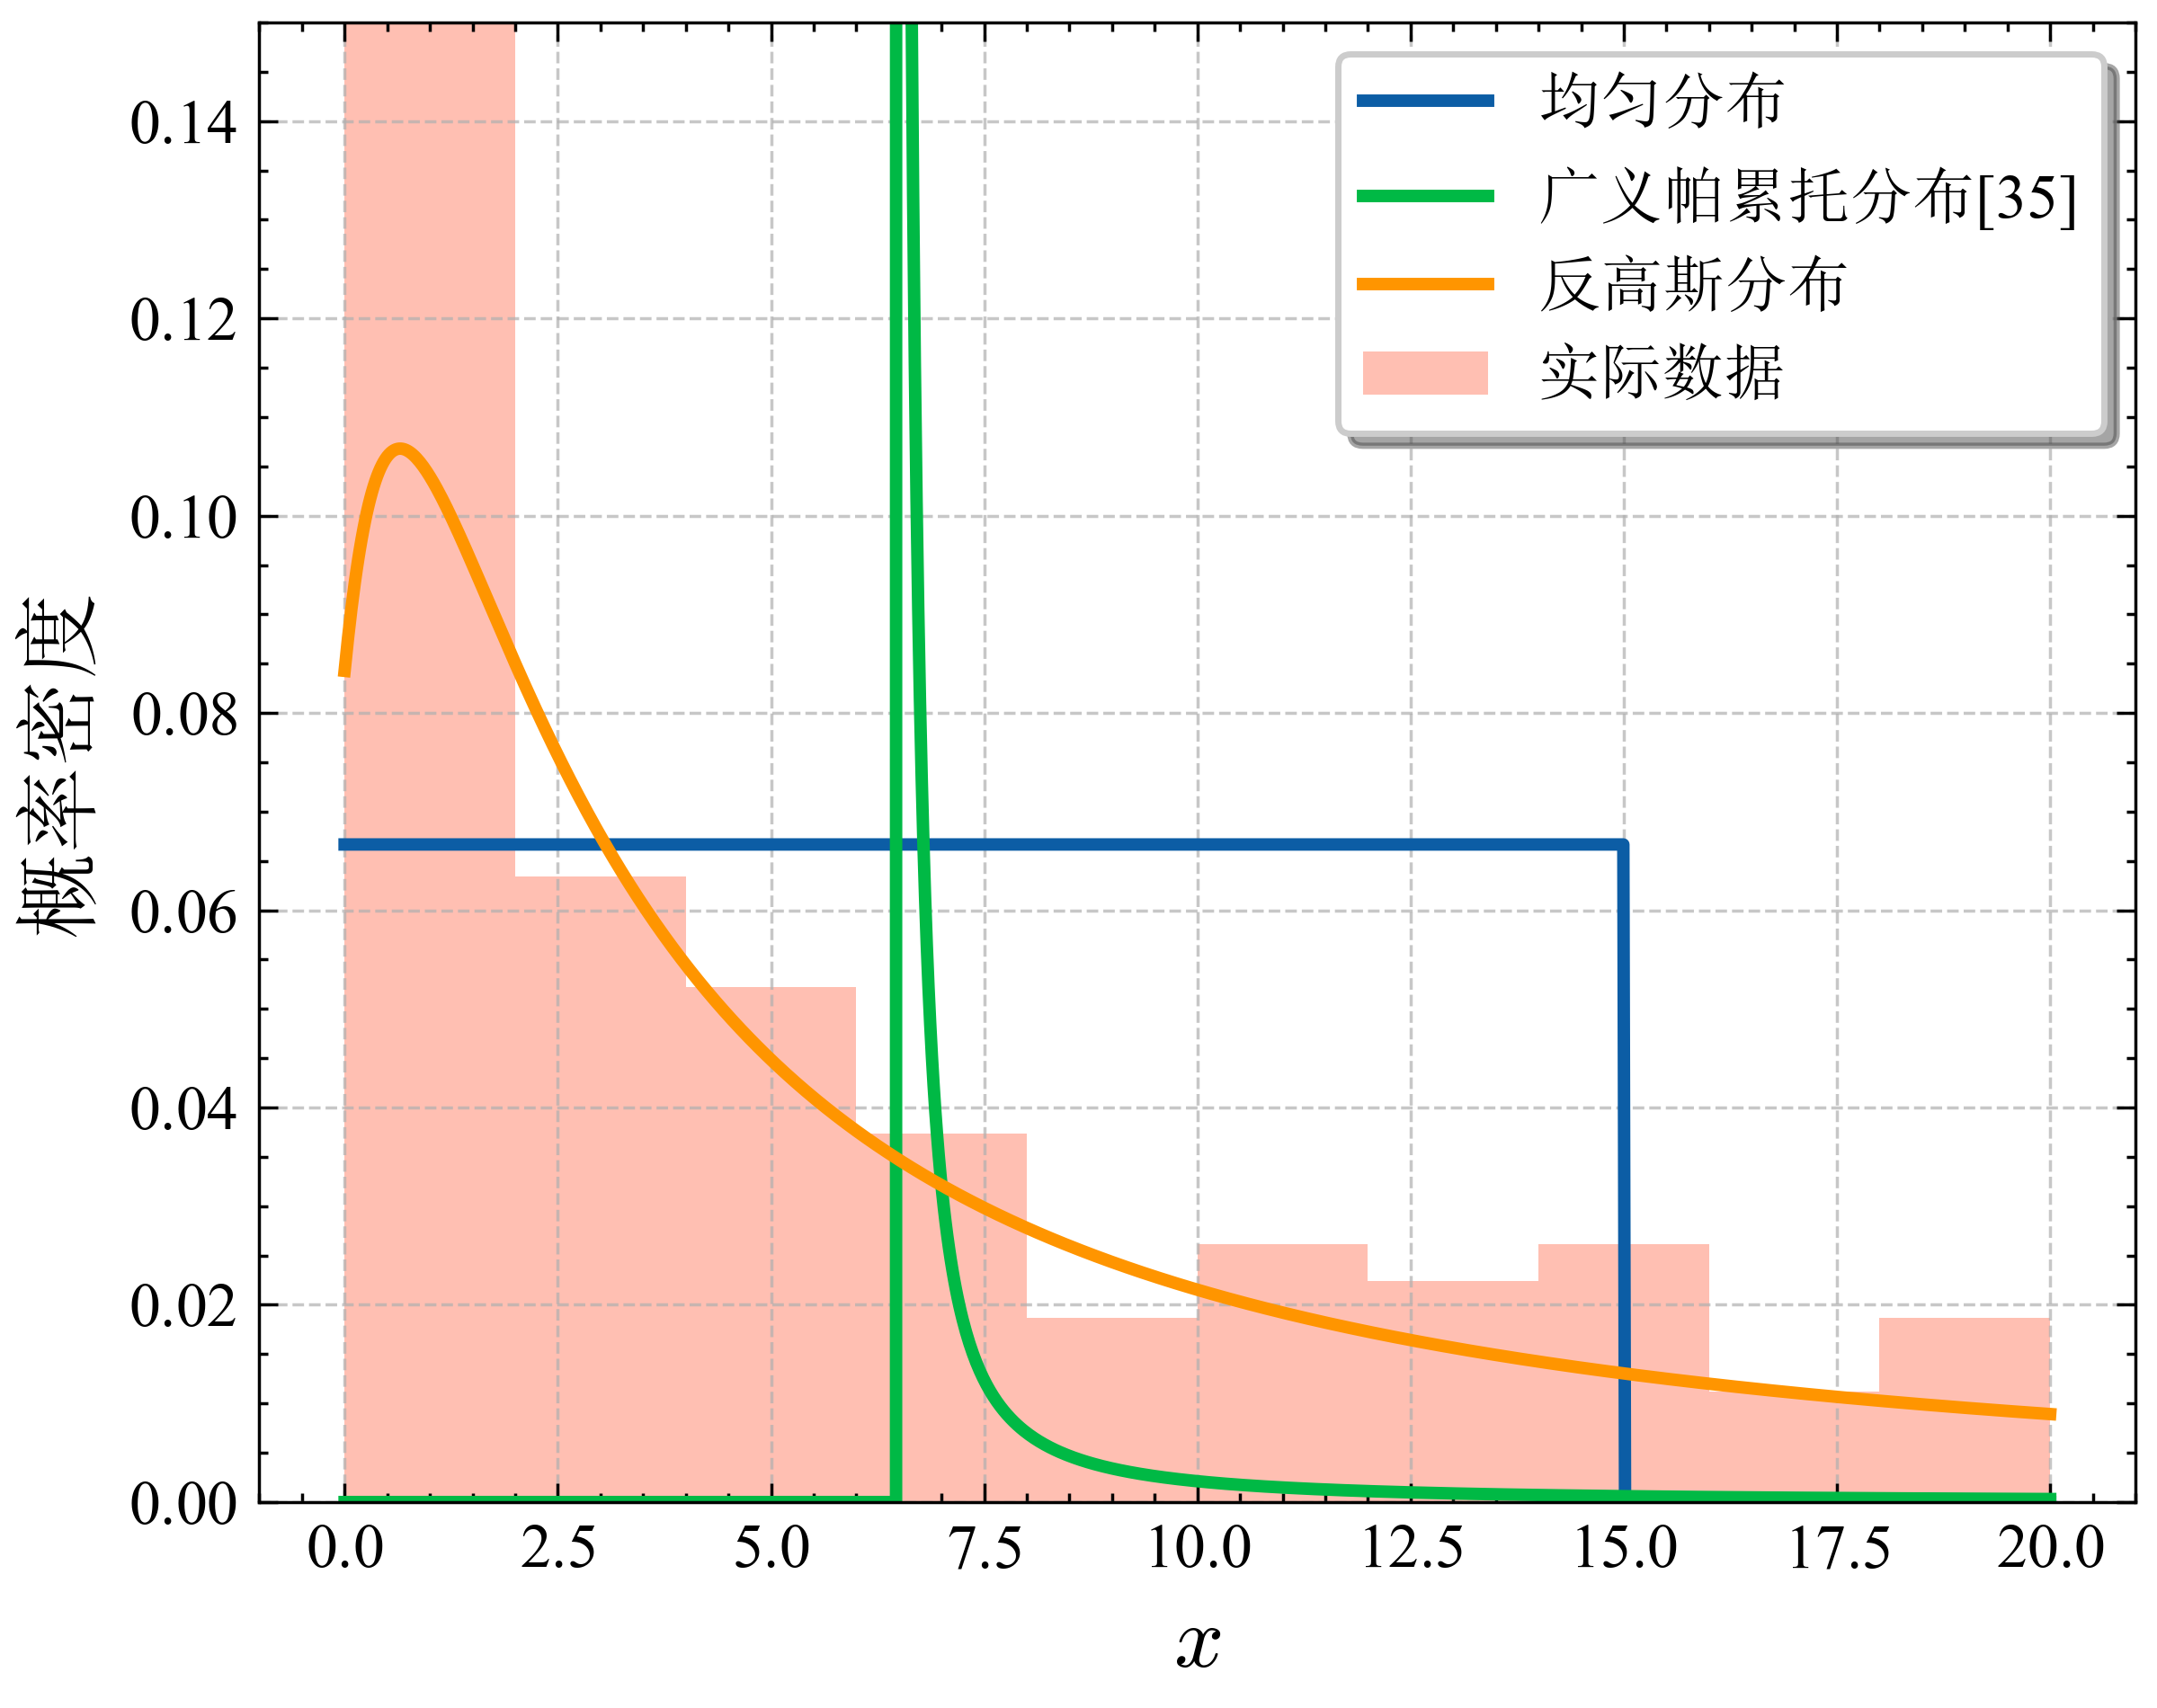
\includegraphics[width=\linewidth]{basic_pictures/分布拟合.png}
            \captionof{figure}{分布拟合结果}
            \label{fig:beamer_dist_fit}
        \end{column}
    \end{columns}
\end{frame}

% \begin{frame}{\insertsectionhead: 不同需求分布下的最优储备结构对比}
%     \begin{figure}
%         \centering
%         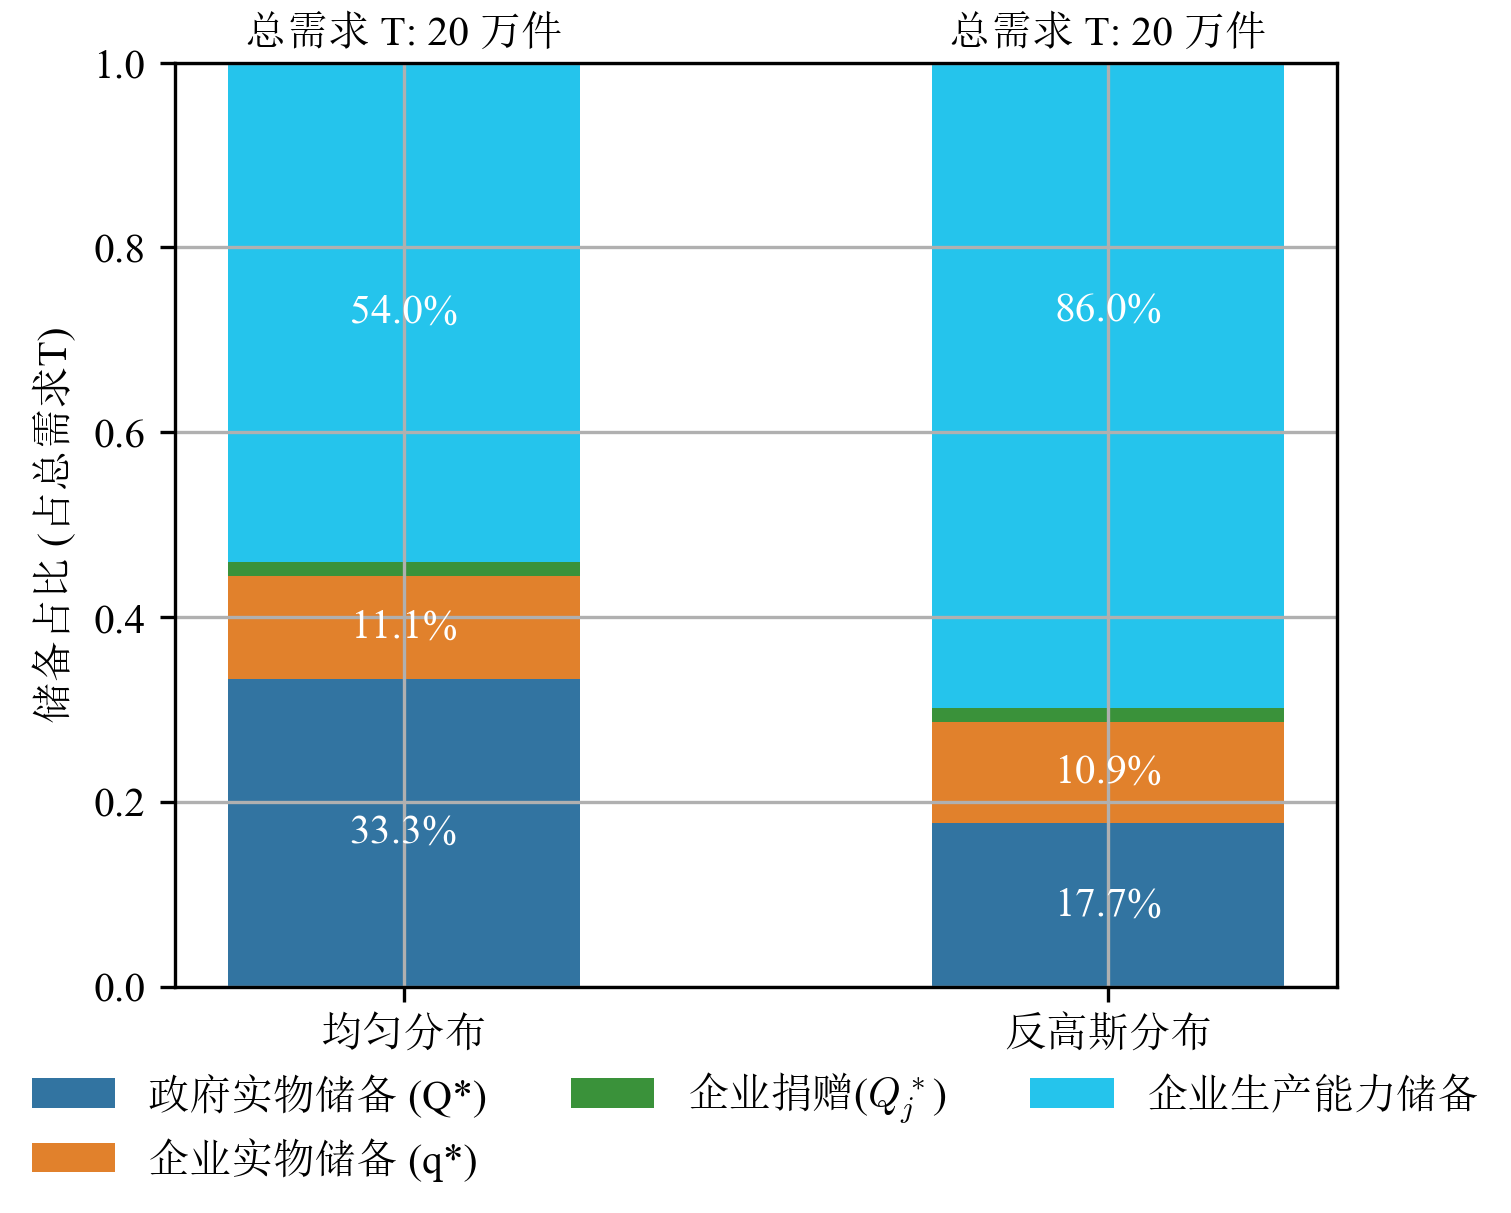
\includegraphics[width=0.7\linewidth]{basic_pictures/储备结构对比.png}
%         \caption{储备结构对比 (U=15万件)}
%         \label{fig:beamer_structure_comparison}
%     \end{figure}
%     \begin{itemize}
%         \item \textbf{均匀分布:} 政府实物(33.3\%), 企业实物(10.3\%), 企业生产(54.3\%)。
%         \item \textbf{反高斯分布:} 政府实物(15.6\%), 企业实物(5.7\%), 更依赖企业生产能力。
%         \item \textbf{启示:} 反高斯分布长尾特性使模型倾向于依赖灾后生产,实物储备起“首轮响应”和“争取时间”作用。
%     \end{itemize}
% \end{frame}

%\begin{frame}{\insertsectionhead: 不同需求分布下的最优储备结构对比}
\begin{frame}{\insertsectionhead: 不同需求分布下的最优储备结构对比}
    \begin{columns}
        % 左边:文字
        \begin{column}{0.5\textwidth}
            \begin{itemize}
                \item \textbf{均匀分布:} 政府实物(33.3\%)、企业实物(10.3\%)、企业生产(54.3\%)。
                \item \textbf{反高斯分布:} 政府实物(15.6\%)、企业实物(5.7\%),更依赖企业生产能力。
                \item \textbf{启示:} 反高斯分布长尾特性使模型倾向于依赖灾后生产,实物储备起“首轮响应”和“争取时间”作用。
            \end{itemize}
        \end{column}

        % 右边:图片
        \begin{column}{0.5\textwidth}
            \centering
            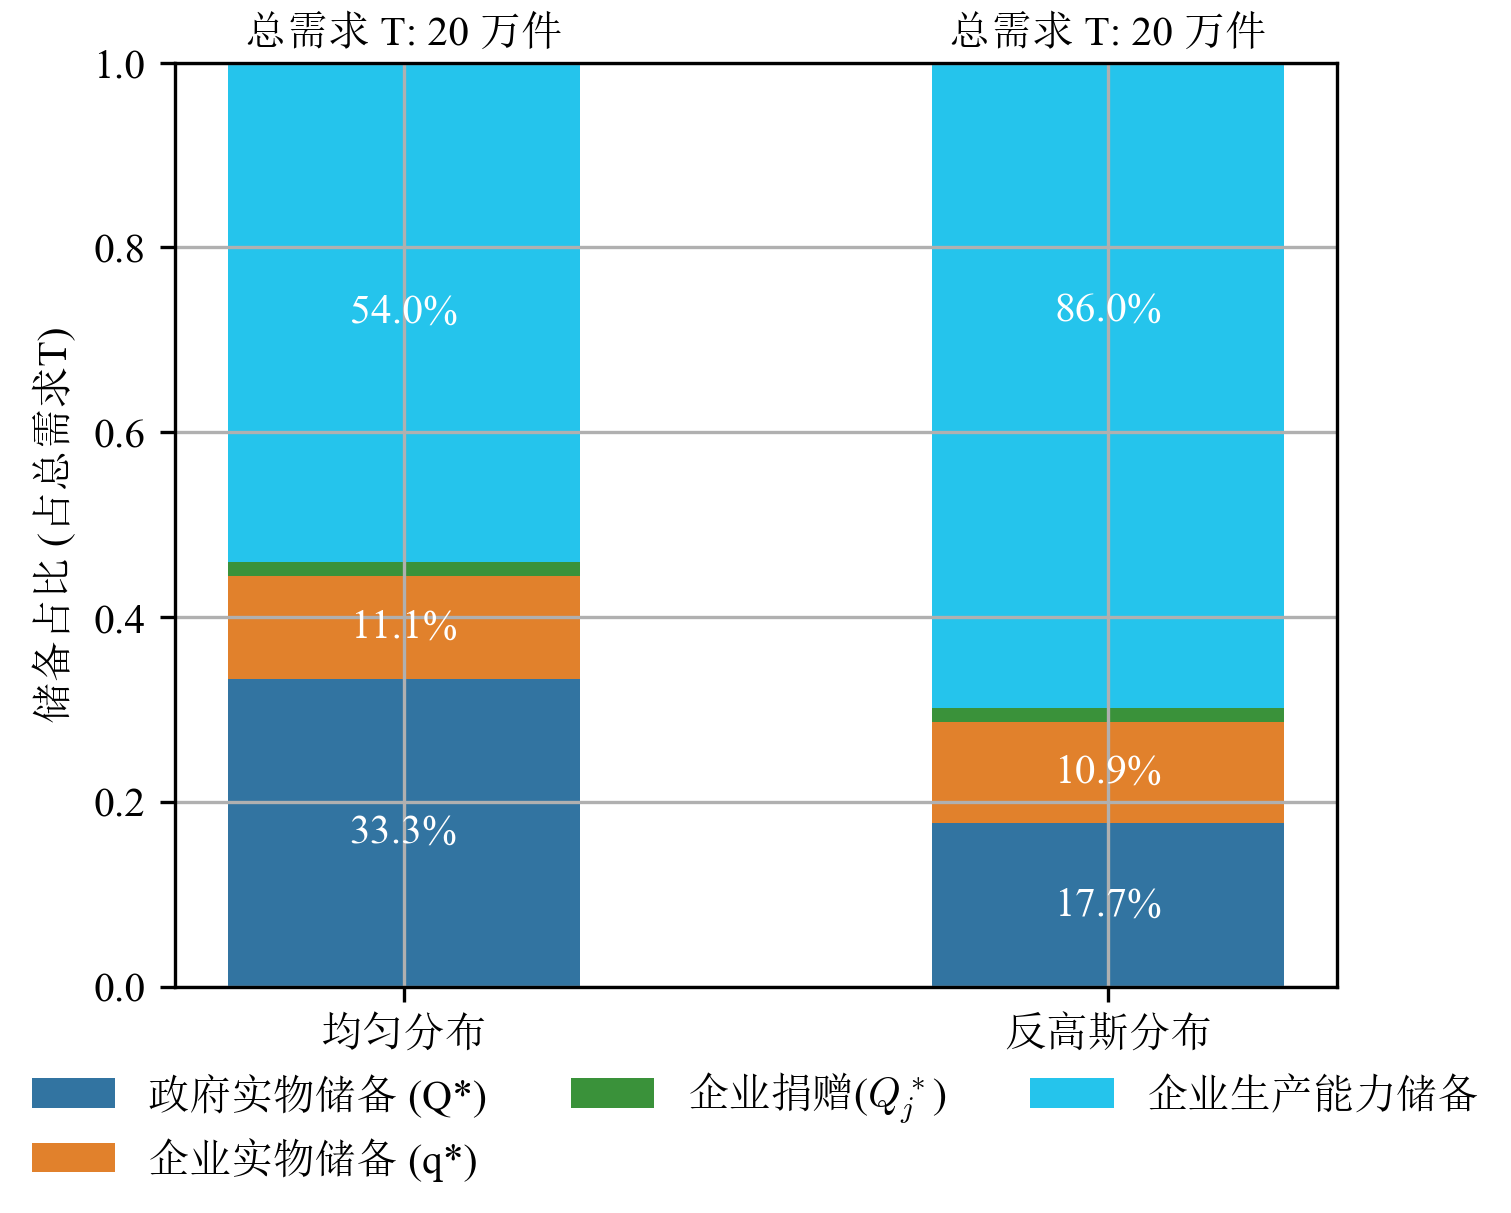
\includegraphics[width=\linewidth]{basic_pictures/储备结构对比.png}
            \vspace{0.5em}

            {\small 图:储备结构对比(U=15万件)}
        \end{column}
    \end{columns}
\end{frame}



\begin{frame}[allowframebreaks]{\insertsectionhead: 不同情景下计算结果}
    \begin{table}
    \centering
    \caption{不同情景下应急物资储备与利润计算结果}
    \tiny % Smaller font for this table
    \begin{tabular}{llrrrrr}
    \toprule
    \textbf{情景} & \textbf{分布} & \textbf{$Q^*$} & \textbf{$q^*$} & \textbf{$p^*$} & \textbf{政府利润} & \textbf{企业利润} \\
    \midrule
    \multirow{2}{*}{基准模型} & 均匀 & 5.00 & 1.54 & 0.31 & -3113.73 & 210.26 \\
     & 反高斯 & 2.34 & 0.85 & 0.31 & -1710.55 & 184.15 \\
    \midrule
    \multirow{2}{*}{不考虑捐赠} & 均匀 & 5.00 & 2.03 & 0.00 & -3197.66 & 288.79 \\
     & 反高斯 & 2.34 & 1.35 & 0.00 & -1767.42 & 238.15 \\
    \midrule
    \multirow{2}{*}{不考虑企业代储} & 均匀 & 6.41 & 0.00 & 0.31 & -3115.91 & 157.06 \\
     & 反高斯 & 3.11 & 0.00 & 0.31 & -1771.28 & 164.47 \\
    \midrule
    \multirow{2}{*}{\begin{tabular}[c]{@{}l@{}}不考虑企业\\代储和生产\end{tabular}} & 均匀 & 7.50 & 0.00 & 0.31 & -3129.75 & 109.95 \\
     & 反高斯 & 39.72 & 0.00 & 0.31 & -6123.92 & 139.60 \\
    \bottomrule
    \end{tabular}
    \end{table}
    \textbf{关键启示:}
    \begin{itemize}
        \item 企业参与能有效分担政府压力,优化储备结构。
        \item 合理的协同契约与激励机制是核心。
        \item 需求特征对最优策略有决定性影响 \cite{LIY2023, zhengh2023, XTGL202004012}。
        \item 多主体协同储备体系能提升保障能力、降低社会总成本。
    \end{itemize}
\end{frame}

\begin{frame}{\insertsectionhead: 敏感性分析 - $m$ 和 $p_1$}
    \begin{columns}[T]
        \begin{column}{0.5\textwidth}
            \textbf{灾害后市场单价 ($m$)影响}
            \begin{figure}
                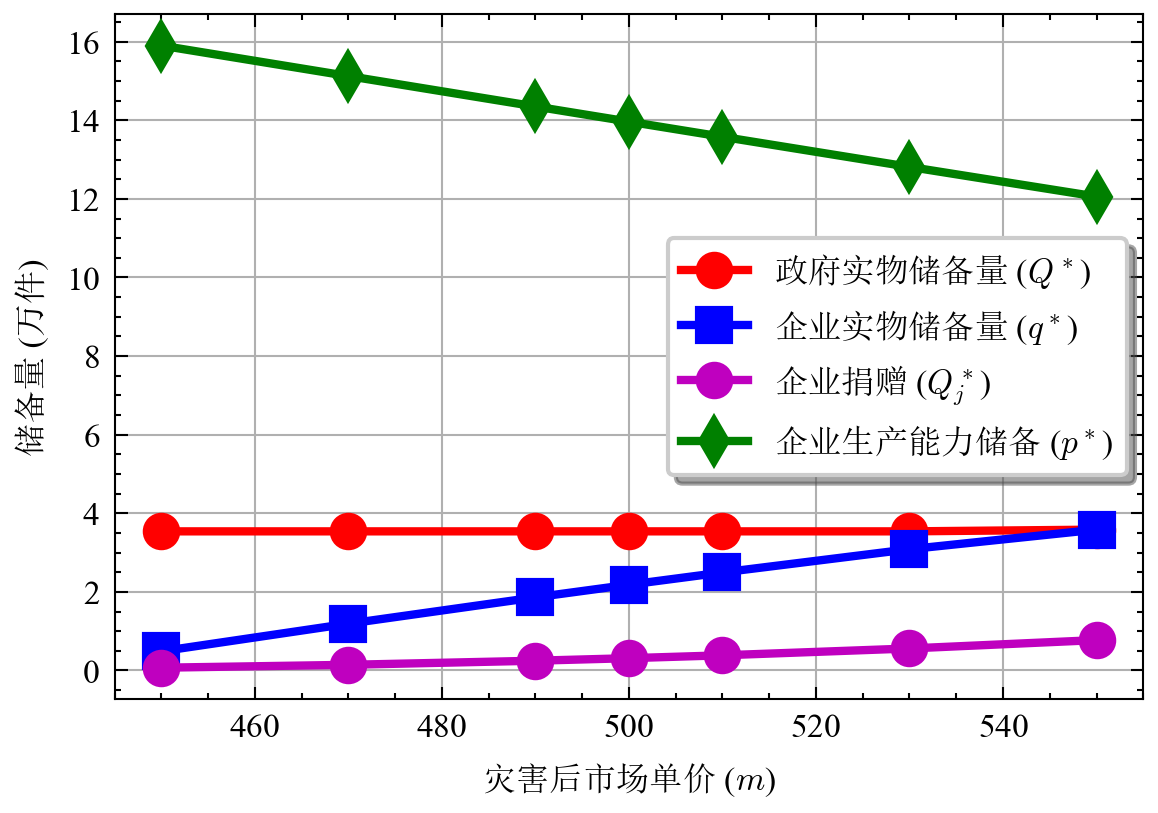
\includegraphics[width=\linewidth]{basic_pictures/sensitivity_m.png}
                \caption*{}
            \end{figure}
            \footnotesize $m \uparrow \implies Q^*$稳定, $q^* \uparrow, Q_j^* \uparrow, p^* \downarrow$
        \end{column}
        \begin{column}{0.5\textwidth}
            \textbf{灾害前物资单价 ($p_1$)影响}
            \begin{figure}
                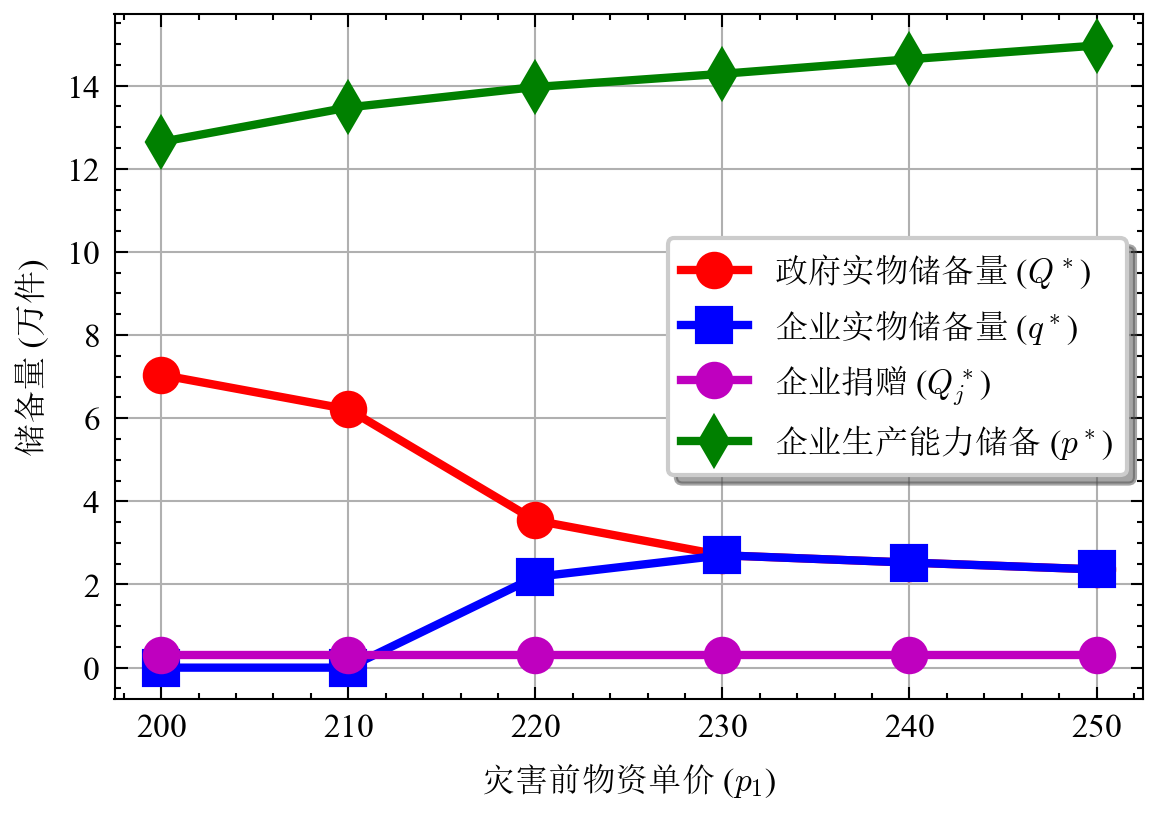
\includegraphics[width=\linewidth]{basic_pictures/sensitivity_p1.png}
                \caption*{}
            \end{figure}
            \footnotesize $p_1 \uparrow \implies Q^* \downarrow, q^*$先增后稳, $p^* \uparrow$
        \end{column}
    \end{columns}
\end{frame}

\begin{frame}{\insertsectionhead: 敏感性分析 - $p_2$ 和 $s$}
    \begin{columns}[T]
        \begin{column}{0.5\textwidth}
            \textbf{企业代储收入 ($p_2$)影响}
            \begin{figure}
                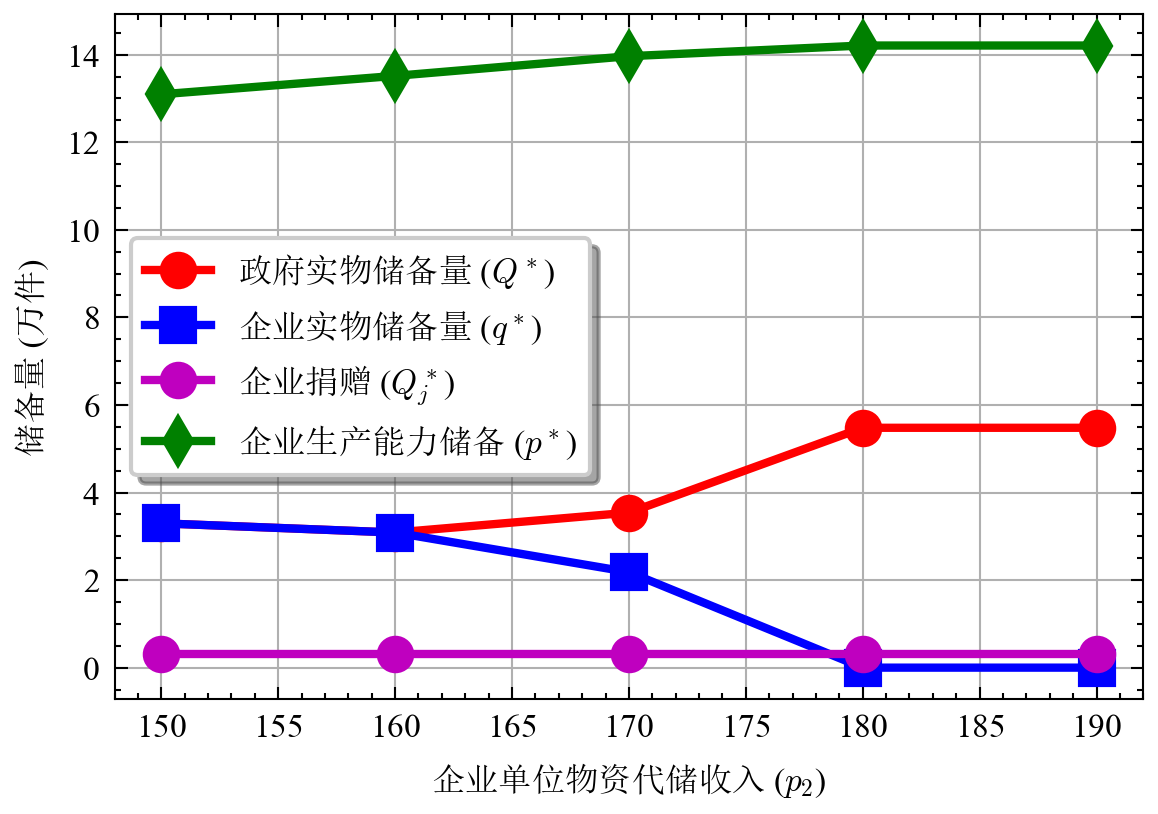
\includegraphics[width=\linewidth]{basic_pictures/sensitivity_p2.png}
                \caption*{}
            \end{figure}
            \footnotesize $p_2 \uparrow \implies Q^*$先稳后增, $q^* \downarrow$ (趋零)
        \end{column}
        \begin{column}{0.5\textwidth}
            \textbf{企业使用补贴 ($s$)影响}
            \begin{figure}
                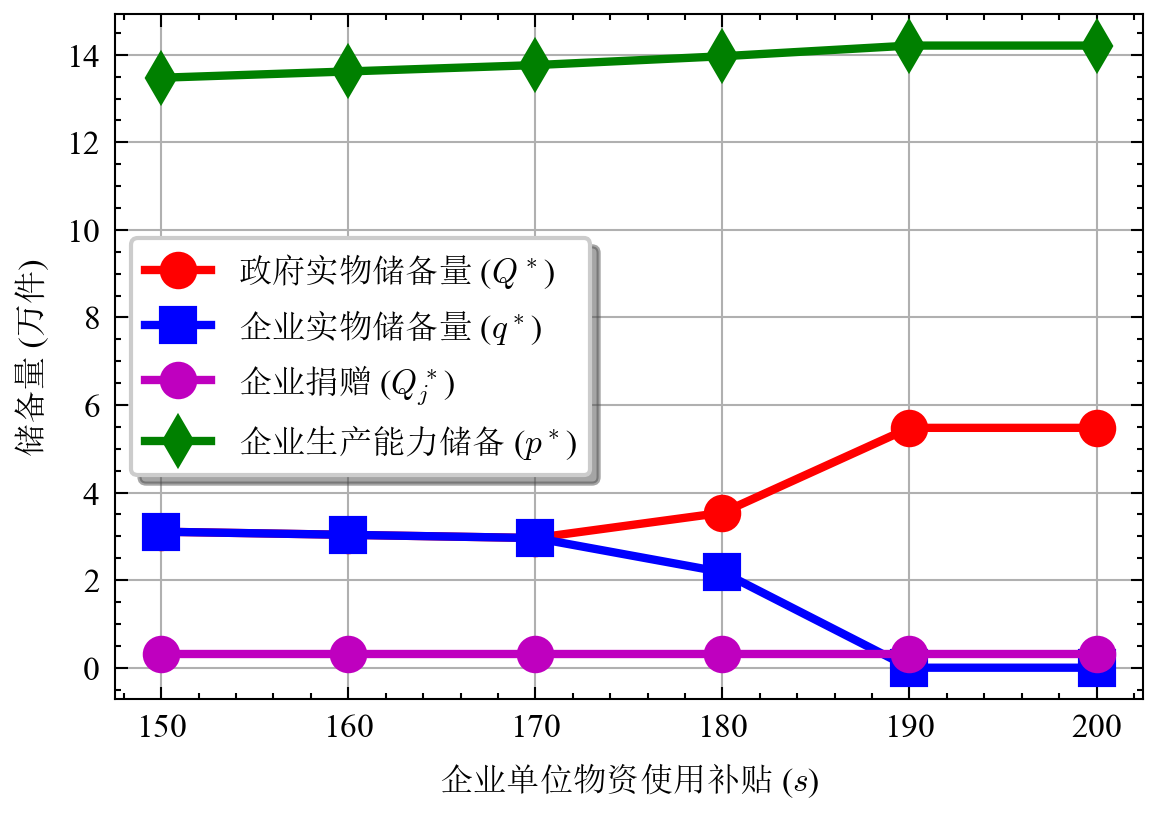
\includegraphics[width=\linewidth]{basic_pictures/sensitivity_s.png}
                \caption*{}
            \end{figure}
            \footnotesize $s \uparrow \implies Q^*$先稳后增, $q^* \downarrow$ (趋零)
        \end{column}
    \end{columns}
\end{frame}

\begin{frame}{\insertsectionhead: 敏感性分析 - $v$ 和 $\alpha$}
    \begin{columns}[T]
        \begin{column}{0.5\textwidth}
            \textbf{单位物资残值 ($v$)影响}
            \begin{figure}
                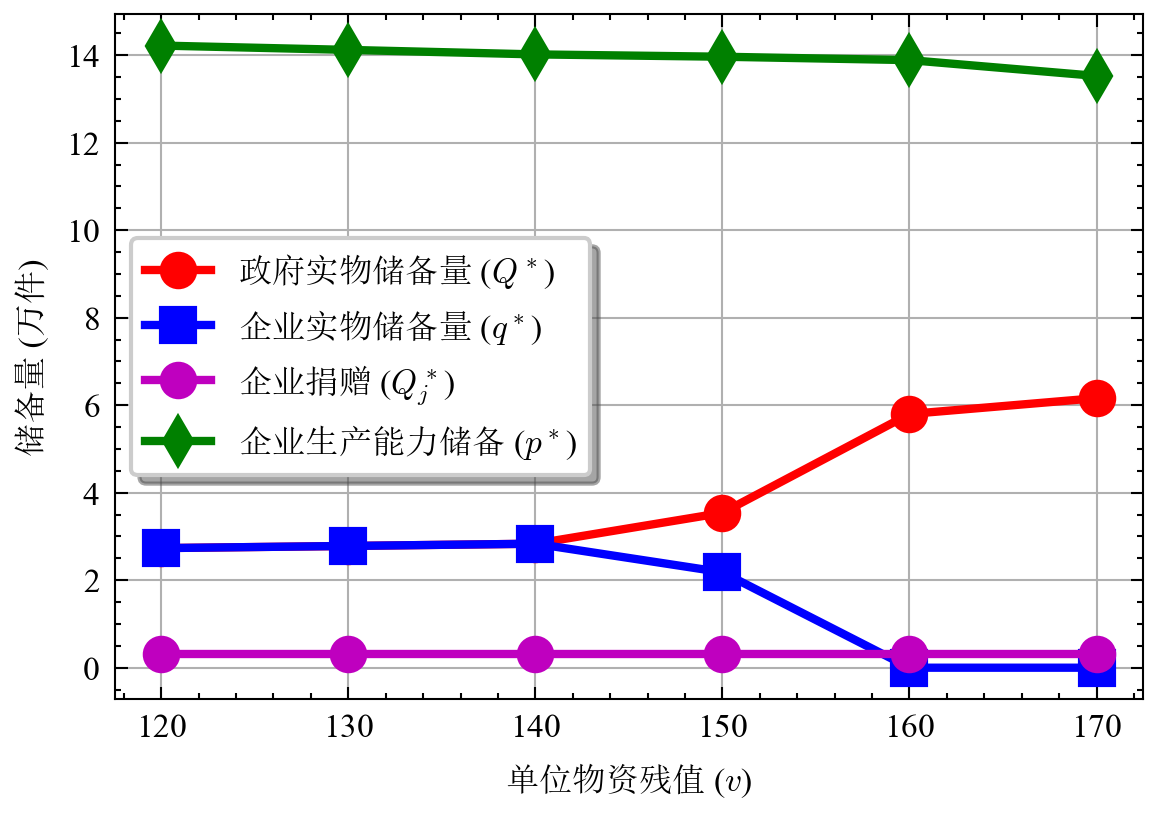
\includegraphics[width=\linewidth]{basic_pictures/sensitivity_v.png}
                \caption*{}
            \end{figure}
            \footnotesize $v \uparrow \implies Q^* \uparrow, q^*$先稳后降 (趋零)
        \end{column}
        \begin{column}{0.5\textwidth}
            \textbf{灾害发生概率 ($\alpha$)影响}
            \begin{figure}
                \includegraphics[width=\linewidth]{basic_pictures/sensitivity_alpha.png}
                \caption*{}
            \end{figure}
            \footnotesize $\alpha \uparrow \implies Q^* \uparrow, q^* \uparrow, p^* \downarrow$
        \end{column}
    \end{columns}
\end{frame}

\begin{frame}{\insertsectionhead: 敏感性分析 - $c_1$ 和 $\lambda$}
    \begin{columns}[T]
        \begin{column}{0.5\textwidth}
            \textbf{政府储存成本 ($c_1$)影响}
            \begin{figure}
                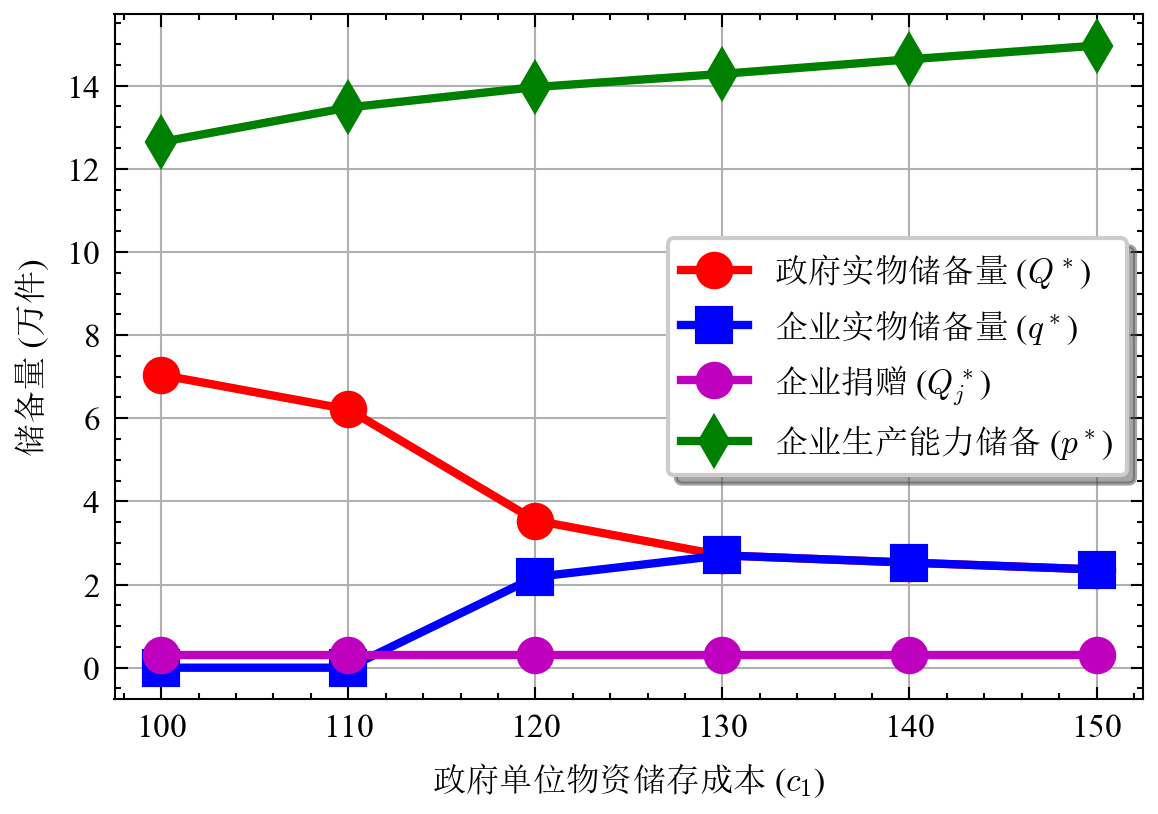
\includegraphics[width=\linewidth]{basic_pictures/sensitivity_c1.png}
                \caption*{}
            \end{figure}
            \footnotesize $c_1 \uparrow \implies Q^* \downarrow, q^*$ ($c_1 \ge 120$后) $\uparrow$后稳
        \end{column}
        \begin{column}{0.5\textwidth}
            \textbf{企业捐赠系数 ($\lambda$)影响}
            \begin{figure}
                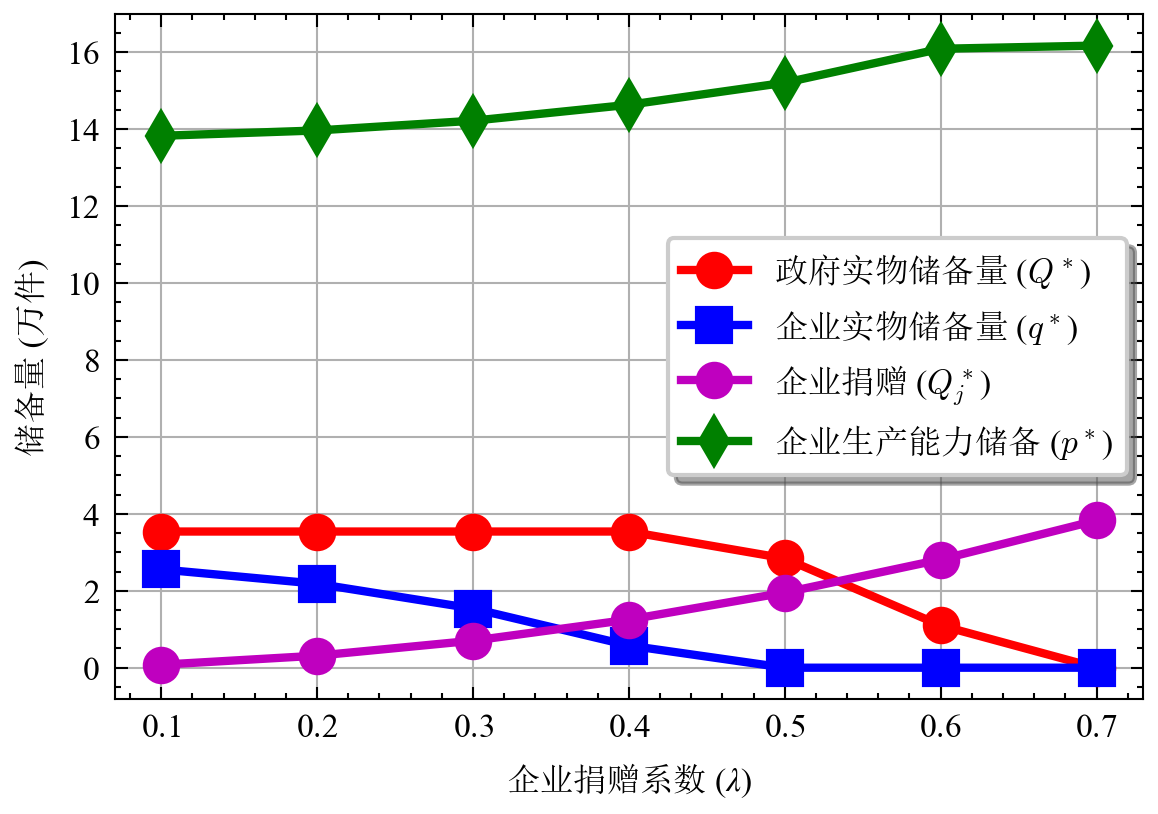
\includegraphics[width=\linewidth]{basic_pictures/sensitivity_lam.png}
                \caption*{}
            \end{figure}
            \footnotesize $\lambda \uparrow \implies Q^*$先稳后降, $q^* \downarrow$ (趋零), $Q_j^* \uparrow$
        \end{column}
    \end{columns}
    \textbf{总结:} 政企决策相互影响,构建有效契约需综合考量各参数。
\end{frame}

\begin{frame}{\insertsectionhead: 算法有效性验证}
    \textbf{参照文献:} 文献 \cite{LIY2023} 中结构简化的模型 (政府实物 + 企业实物 + 企业生产)。
    \begin{itemize}
        \item 本文模型设置 $\lambda=0$ (无捐赠) 以对标。
    \end{itemize}
    \begin{table}
    \centering
    \caption{SLSQP算法求解结果与文献精确解对比}
    \small
    \begin{tabular}{clccc}
    \toprule
    分布类型 & 决策变量 & 文献精确解 & SLSQP数值解 & 相对误差 (\%) \\
    \midrule
    \multirow{2}{*}{均匀分布 (UD)} & $Q^*$ & 2082 & 2081.6188 & 0.0183 \\
    & $q^*$ & 520  & 520.4230  & 0.0813 \\
    \midrule
    \multirow{2}{*}{广义帕累托分布 (GPD)} & $Q^*$ & 679 & 678.8855 & 0.0169 \\
    & $q^*$ & 346 & 345.1098 & 0.2573 \\
    \bottomrule
    \end{tabular}
    \end{table}
    \textbf{结论:}
    \begin{itemize}
        \item SLSQP算法数值解与精确解高度吻合。
        \item 相对误差极小,验证了算法的有效性和准确性。
    \end{itemize}
\end{frame}

\section{结论与未来展望}
\begin{frame}{\insertsectionhead: 主要结论}
    \begin{enumerate}
        \item \textbf{需求分布影响显著:} 反高斯分布更贴近现实,优化储备结构,降低政府开支。
        \item \textbf{灾害概率与捐赠意愿:} 灾害概率增加促使实物储备增加;企业捐赠主要受捐赠效益系数影响。
        \item \textbf{政企决策相互影响:} 政府成本、企业代储收入/补贴等参数均影响双方决策平衡点。
        \item \textbf{市场价格与残值:} 其增加会降低实物储备净成本,促使增加实物储备。
        \item \textbf{算法有效性:} SLSQP算法能有效准确求解模型。
    \end{enumerate}
\end{frame}

\begin{frame}{\insertsectionhead: 管理启示}
    \begin{itemize}
        \item 应急储备规划应考虑需求分布长尾特性,避免资源浪费。
        \item 政府应加强实物储备,并通过激励机制鼓励企业履行社会责任 (如捐赠)。
        \item 设计政企合作契约时,需平衡各方利益,合理设置费用和补贴。
    \end{itemize}
\end{frame}

\begin{frame}{\insertsectionhead: 研究不足与未来展望}
    \textbf{不足之处:}
    \begin{itemize}
        \item 未考虑需求动态变化。
        \item 未区分不同类型物资。
        \item 未考虑多层级供应链结构。
    \end{itemize}
    \textbf{未来研究方向:}
    \begin{itemize}
        \item 构建更复杂、贴近实际的应急物流储备模型。
        \item 探索更精巧的契约机制设计。
        \item 提升应急物资保障体系的韧性和效率。
    \end{itemize}
\end{frame}

\begin{frame}[allowframebreaks]{参考文献}
    \renewcommand*{\bibfont}{\footnotesize}

    \printbibliography
\end{frame}

\end{document}
